\begin{figure}
\centering
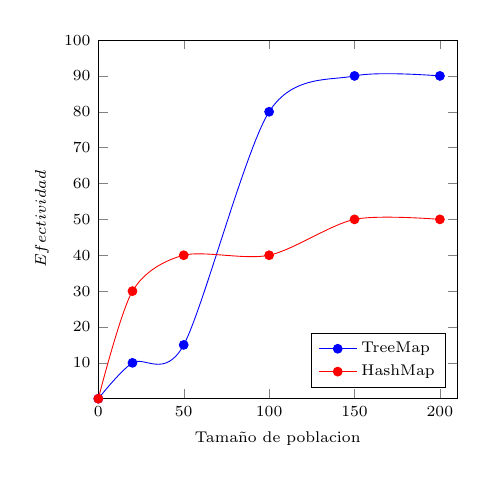
\begin{tikzpicture}[scale=0.8]
\begin{axis}[
    width=0.60\textwidth,
    height=0.60\textwidth,
    xmin=0, xmax=210,
    ymin=0, ymax=100,
    xlabel={\scriptsize{Tamaño de poblacion}},
    ylabel={\scriptsize{$Efectividad$}},
    xtick={0,50,...,200},
    ytick={10,20,...,100},
    legend pos=south east,
    legend cell align={left},
    legend style={font=\scriptsize},
    tick label style={font=\scriptsize}
]

\addplot[mark=*,blue,,smooth] coordinates {
    (0, 0)
    (20, 10)
    (50, 15)
    (100, 80)
    (150, 90)
    (200, 90)

  
};

\addplot[mark=*,red,,smooth] coordinates {
    (0, 0)
    (20, 30)
    (50, 40)
    (100, 40)
    (150, 50)
    (200, 50)

  
};
\legend{TreeMap,HashMap}
\end{axis}
\end{tikzpicture}%
\hfill
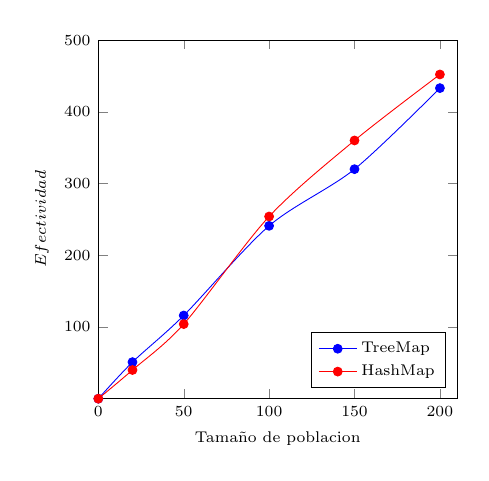
\begin{tikzpicture}[scale=0.8]
\begin{axis}[
    width=0.60\textwidth,
    height=0.60\textwidth,
    xmin=0, xmax=210,
    ymin=0, ymax=500,
    xlabel={\scriptsize{Tamaño de poblacion}},
    ylabel={\scriptsize{$Efectividad$}},
    xtick={0,50,...,200},
    ytick={100,200,...,500},
    legend pos=south east,
    legend cell align={left},
    legend style={font=\scriptsize},
    tick label style={font=\scriptsize}
]

\addplot[mark=*,blue,,smooth] coordinates {
    (0, 0)
    (20, 51)
    (50, 116)
    (100, 241)
    (150, 320)
    (200, 433)

  
};

\addplot[mark=*,red,,smooth] coordinates {
    (0, 0)
    (20, 40)
    (50, 104)
    (100, 254)
    (150, 360)
    (200, 452)

  
};
\legend{TreeMap,HashMap}


\legend{TreeMap, HashMap}

\end{axis}
\end{tikzpicture}

\caption{Gráficos de Efectividad y cantidad de candidatos de acuerdo al rate de mutación}
\end{figure}

